\chapter{Evaluation and Discussion}

In this chapter we explain our experiment and present the results obtained from our models for the problem of finding Trustworthy and Untrustworthy content on Twitter. We then discuss and generally reflect on the results obtained.

\section{Experiment}
In this section we detail our experiment and data statistics. The table below gives an overview of the variety of our data. 
\begin{center}
\captionof{table}{Data Statistics} 
\begin{tabular}{|l|l|}
\hline
Total Number of Tweets  &  17203  \\ \hline
Total Number of Unique Users & 45  \\ \hline
Number of Trustworthy Users  & 20 \\ \hline
Number of Untrustworthy Users & 25  \\ \hline
Number of Retweets   & 15364  \\ \hline
Number of non-Retweets & 2839  \\ \hline
Tweets with No Emotion &  16932\\ \hline
Happy Tweets   & 139 \\ \hline
Sad Tweets    & 132 \\ \hline
Tweets that are Replies & 381 \\ \hline
Tweets that are not replies & 16278 \\ \hline
 Features : DataPoints & 29 : 17203  \\ \hline
\end{tabular}
\end{center}
As with any Machine Learning problem, our training and testing cycle utilises a trial and error approach. This consists of training multiple data sets with data points being collected at varying points in time. The aim of this approach is to increase the performance of models on each subsequent iteration. For this task we used 80\% of the data to train the three different classifiers separately and used the remaining 20\% of the data to test the performance of our models. We also independently evaluated the results, using a raw data set which was not related to the previous dataset. That is, it consisted entirely of new tweets from new users. We hand picked some known fake tweets, particularly ones that arise during crisis situations (Tweets that have been repeatedly reported in news paper articles and other research papers) as our Untrustworthy tweets and some tweets from other news agencies for our Trustworthy tweets. This dataset consisted of 39 tweets, 20 being Untrustworthy and 19 being Trustworthy. However, we also wanted to test our model on general tweets by the average user, so we evaluated the performance of the model on a much smaller dataset of 12 tweets of which all of them but one were Trustworthy. In the next paragraph we go into detail about the parameters used in our Machine Learning models.\\*\\*
For our Logistic Regression (LR) classifier we used an L2 regularisation parameter, which is essentially a parameter that we pass into our model, which reduces overfitting $LR(L_2)$. In the case of Support Vector Machines (SVM) as mentioned in Chapter 5, we used a Radial Basis Function (\textit{rbf}) kernel. We also tried using Linear and Polynomial kernels however the best performance was achieved with \textit{rbf}. For SVM, there are two important parameters that needs to be specified. They are $C$ and $gamma$. The parameter $C$ trades off misclassification of training data against a simple decision surface [39]. $C$, when low would give a smooth decision surface, whereas when high it aims to classify all training samples correctly thereby not producing a smooth decision surface. The gamma value determines the level of influence of a single training sample. If the $gamma$ is large, then the samples should be closer to each other to be affected \cite{39}. We used 1 for $C$ and 0 for $gamma$. It is usually a good idea to change these values around to get a better decision surface. \\*\\*
In the case of the Random Forests (RF) classifier, we had to specify the number of trees we want in our model; in our case we specified 500. This is because the number of trees, is not a tuning parameter in RF. Although a high number of trees is usually always better, once we have enough trees to work with the accuracy doesn't improve, hence it would be computationally wasteful to specify more than the necessary number of trees. However in our case we used 500 as this gave us quality predictions. We used information gain\footnote{Calculates how much information we gained by doing the slicing on this particular node or feature}as the quality of our split since the gini index\footnote{The attribute value that provides the smallest split is chosen as the node to split on} gave us slightly poor performance. 
\section{Results}
In this section we present the results obtained from the three different classifiers used in our experiment above. In the following subsections we discuss accuracy, precision, recall and Area Under Curve (AUC) all of which are measurements used to measure the ability of the model to predict appropriately. 
\subsection{Accuracy, Precision and Recall}
In order to understand this section, the reader needs a clear idea of what some of the metrics we calculated represent. The table given below addresses that.\\*\\*
\begin{minipage}{\linewidth}
\centering
\captionof{table}{Measurements}
\begin{tabular}[t]{|C{.90in}|C{3.00in}|C{1.60in}|}
\toprule[1.5pt]
Measure & Explanation & Formula\\\midrule
True Positive & Correctly classified as Trustworthy - Trustworthy Tweet & TP \\
\hline
False Positive & Incorrectly classified as Trustworthy - Untrustworthy Tweet & FP \\
\hline   
True Negative & Correctly classified as Untrustworthy - Untrustworthy Tweet & TN\\
\hline
False Negative & Incorrectly classified as Untrustworthy - Trustworthy Tweet & FN\\
\hline
TPR & True Positive Rate & $\frac {TP}{TP + FN}$\\
\hline 
FPR & False Positive Rate &  $\frac {FP}{FP + TN}$\\
\hline
TNR & True Negative Rate &  $\frac {TN}{FP + TN}$\\
\hline
FNR & False Negative Rate & $\frac {FN}{TP + FN}$\\
\hline
Accuracy & The degree of closeness of measurements to the actual value &  $\frac {TP + TN}{TP + FP + FN + TN}$  \\    
\hline
Precision & The precision is the fraction of the retrieved values which are relevant  &  $\frac{TP}{TP + FP}$\\
\hline
Recall &  The recall is the fraction of relevant instances received &  $\frac{TP}{TP+FN}$\\
\hline
$F_\beta$ & This is the harmonic mean of precision and recall. We used the value `1' for $\beta$ & $(1 + \beta^2)\frac{Precision \times Recall}{\beta^2 Precision + Recall}$\\
\hline      
Support & The number of occurrences of each classification label in in truth & - \\
\hline                                                                                                                                                                                    
\bottomrule[1.25pt]
\end{tabular}
\label{tab:LPer}
\end{minipage}
\newpage
\noindent
The following table gives us the accuracy scores of each of the classifiers. As we can see from the table, RF seems to have been performing quite well on Training, Test and the new Data Set however, has performed slightly poorly in comparison to the other techniques when it tested with some random tweets from the average user. Logistic Regression, has performed quite well on all four data sets. The problem with the accuracy score is that the two different outcomes (Trustworthy and Untrustworthy) are not necessarily equal in weight. For example, if our classifier predicted that a tweet is Untrustworthy but it is, in actuality Trustworthy then this would not be much of an issue. However, if our classifier predicted an Untrustworthy tweet as Trustworthy then this might be a problem, since this is exactly how rumours spread.  \\*\\*
\begin{minipage}{\linewidth}
\centering
\captionof{table}{Accuracy} \label{tab:title} 
\begin{tabular}[t]{ C{1.4in} *3{C{1.4in}}}\toprule[1.5pt]
\bf Data & \bf Logistic Regression & \bf Support Vector Machines & \bf Random Forests \\\midrule
Training        &  0.99651  & 1.0 & 1.0\\
Test        &  0.99709     & 0.90380 & 1.0 \\
New Data        &  0.87179   & 0.48717  & 0.97435 \\
Random New Data & 0.83333 & 0.91666 & 0.41666 \\ 
\bottomrule[1.25pt]
\end {tabular}\par
\bigskip
\end{minipage}\\*\\*
\noindent
For precisely the reasons mentioned above we will look at further ways of measuring the quality of our model. Figures 6.1, 6.2 and 6.3 below, show a confusion matrix. A confusion matrix is a nice way of visualising the predictions of a classifier. The $x-axis$ represents the true values of the data points and the $y-axis$ represents the predictions made by the classifiers. We show the confusion matrix for the training data in the diagrams below, however the matrix of the new dataset and the random new dataset can be found in the appendix. In this matrix data points belonging to coordinates $(0,0) , (1,1)$ are correctly classified and points that fall in the $(0,1) , (1,0)$ box are incorrectly classified. One way to look at this matrix would be,\textit{ `When a tweet is Trustworthy, how often do our models classify this correctly?'}. A measure such as this is called `Recall' and by looking at the three diagrams below we can see that SVM and Random Forests have a high recall score (They predict 2293 times correctly out of the total of 2293). The other question we could ask to understand this diagram is \textit{`When our model predicts that a tweet is Trustworthy, how often is it actually Trustworthy?'}. This is known as the precision. Looking at our diagrams we could say that Random Forests give us the best score here as it correctly predicts 2293 out of 2293 instances, where as the LR and SVM fall behind by 2292 out of 2299 and 2293 out of 2624 respectively. In tables 6.4 and 6.5 we show the precision and recall measures for our different datasets.   \\*\\*

\begin{minipage}{\linewidth}
\centering
\captionof{table}{Precision} \label{tab:title} 
\begin{tabular}[t]{ C{1.4in} *3{C{1.4in}}}\toprule[1.5pt]
\bf Data & \bf Logistic Regression & \bf Support Vector Machines & \bf Random Forests \\\midrule
Training        &  0.99528  & 1.0 & 1.0\\
Test        &  0.99608     & 0.87385 & 1.0 \\
New Data        &  0.84999   & 0.48717  & 0.95000 \\
Random New Data & 1.0 & 0.91666 & 1.0 \\ 
\bottomrule[1.25pt]
\end {tabular}\par
\bigskip
\end{minipage}\\*\\*

\begin{minipage}{\linewidth}
\centering
\captionof{table}{Recall} \label{tab:title} 
\begin{tabular}[t]{ C{1.4in} *3{C{1.4in}}}\toprule[1.5pt]
\bf Data & \bf Logistic Regression & \bf Support Vector Machines & \bf Random Forests \\\midrule
Training        & 0.99956  & 1.0 & 1.0\\
Test        &  0.99956     & 1.0 & 1.0 \\
New Data        &  0.89473  & 1.0  & 1.0 \\
Random New Data & 0.90000 & 1.0 & 0.36363 \\ 
\bottomrule[1.25pt]
\end {tabular}\par
\bigskip
\end{minipage}\\*\\*

\begin{figure}[!h]
  \centering
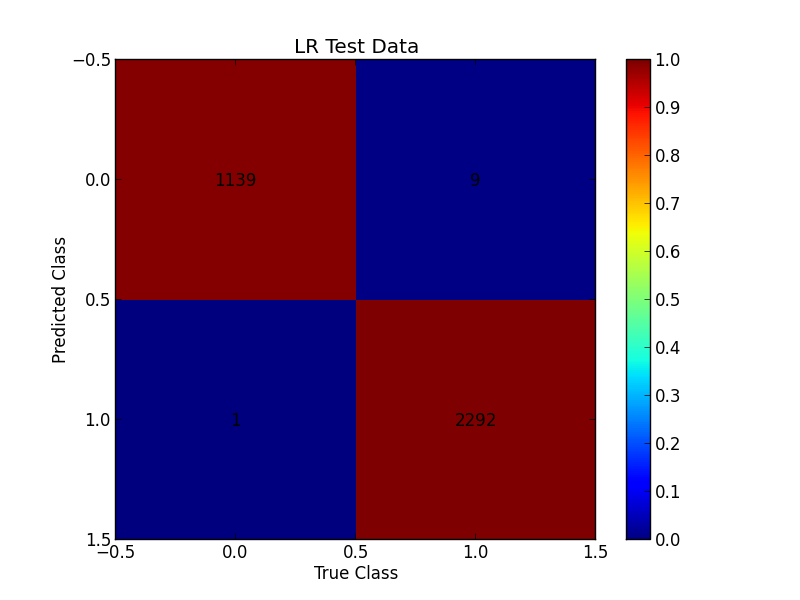
\includegraphics[width=10cm]{LRCMTestData}
  \caption[Logistic Regression Confusion Matrix]
   {Logistic Regression Confusion Matrix}
\end{figure}

\begin{figure}[!h]
 \centering
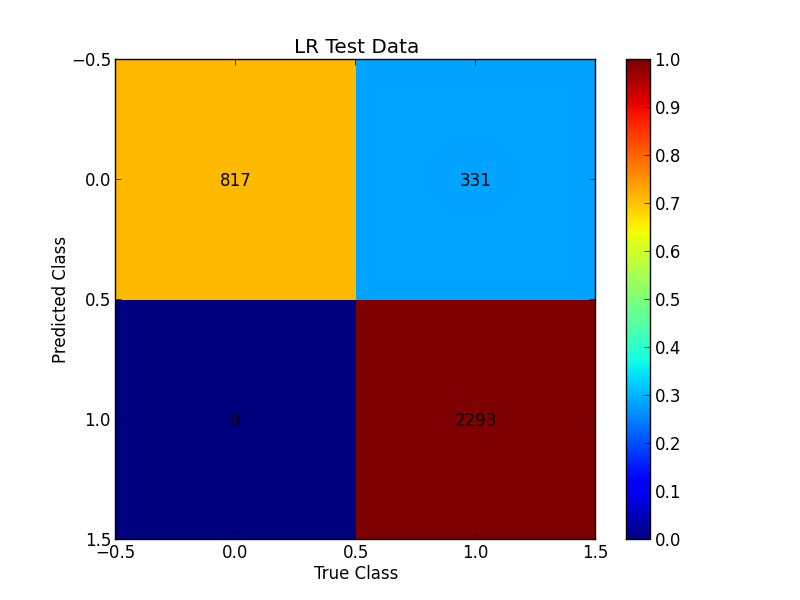
\includegraphics[width=10cm]{SVMCMTestData}
  \caption[Support Vector Machine Confusion Matrix]
   {Support Vector Machine Confusion Matrix}
\end{figure}

\begin{figure}[!h]
 \centering
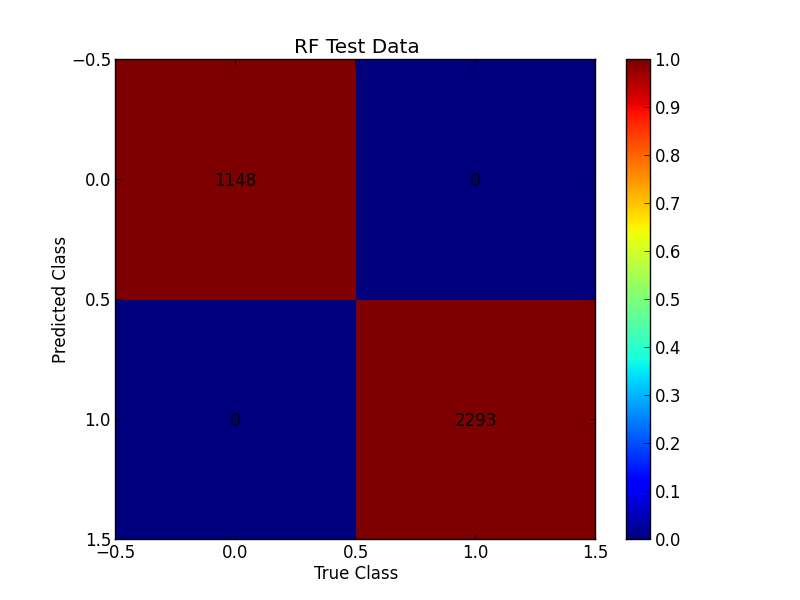
\includegraphics[width=10cm]{RFCMTestData}
  \caption[Random Forests Confusion Matrix]
   {Random Forests Confusion Matrix}
\end{figure}

\subsection{Probabilities}
Delving further into measuring the quality of our system, sometimes decision making can favour a probability estimation over a simple classification. In some cases it makes more sense to say `\textit{This person has a 90\% chance to pass the exam}' as opposed to saying `\textit{You will pass}'. However assessing how good a model is when we have probabilities as opposed to classifications could be quite difficult. Ergo we predict the probabilities of a tweet being Trustworthy or not then calculate the TPR and FPR and plot this on a graph. The graph below plots the TPR values on the $x-axis$ and FPR values on the $y-axis$. The top left corner of the graph is the most ideal point since it has a FP rate of 0 and a TP rate of 1. We ideally want to maximise the TPR while minimising the FPR. AUC, is the area under the curve, which essentially refers to the area within the curve created by out plot. We therefore aim to achieve a high AUC score. The table 6.6 gives the AUC scores of our classifiers and the figures 6.4,6.5 and 6.6 below demonstrate the AUC for our different datasets. \\*\\*

\begin{minipage}{\linewidth}
\centering
\captionof{table}{Area Under Curve} \label{tab:title} 
\begin{tabular}[t]{ C{1.4in} *3{C{1.4in}}}\toprule[1.5pt]
\bf Data & \bf Logistic Regression & \bf Support Vector Machines & \bf Random Forests \\\midrule
Test        &  0.99999     & 0.99742 & 1.0 \\
New Data        &  0.94342  & 0.5000  & 0.97632 \\
Random New Data & 1.0 & 0.5000 & 1.0 \\ 
\bottomrule[1.25pt]
\end {tabular}\par
\bigskip
\end{minipage}\\*\\*

\begin{figure}[!h]
 \centering
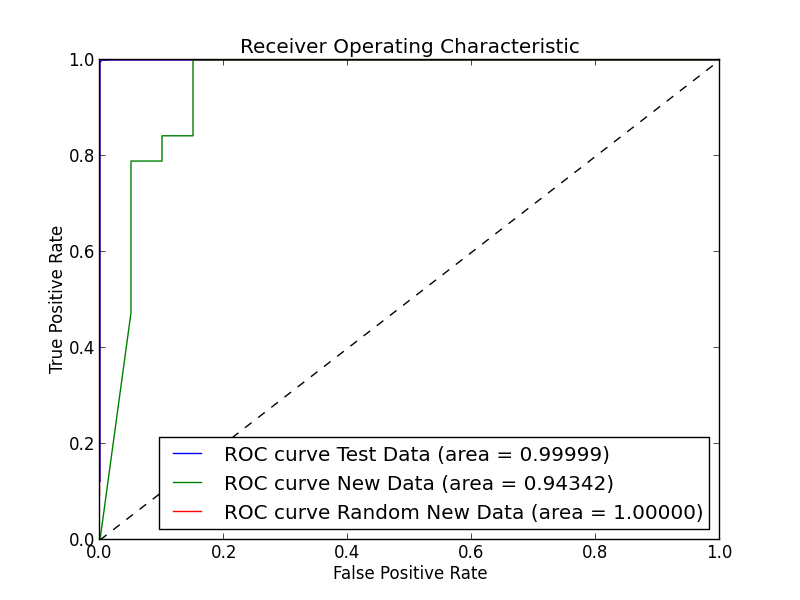
\includegraphics[width=10cm]{LRROCAUC}
  \caption[Logistic Regression AUC]
   {LR ROC Area Under Curve}
\end{figure}

\begin{figure}[!h]
 \centering
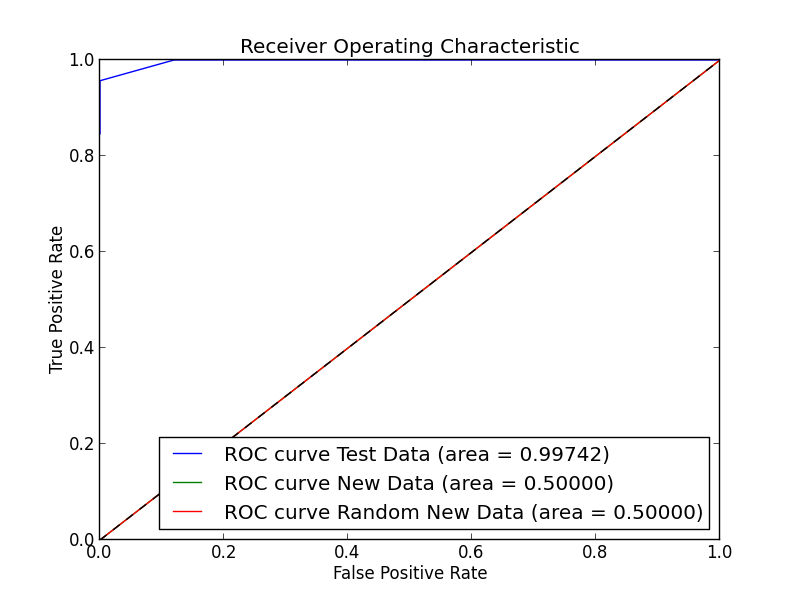
\includegraphics[width=10cm]{SVMROCAUC}
  \caption[Support Vector Machine AUC]
   {SVM ROC Area Under Curve}
\end{figure}

\begin{figure}[!h]
 \centering
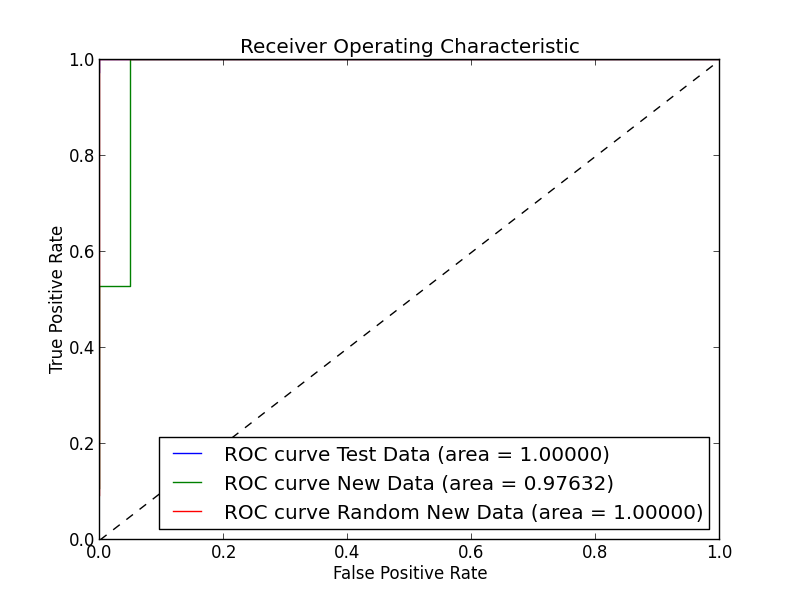
\includegraphics[width=10cm]{RFROCAUC}
  \caption[Random Forests AUC]
   {RF ROC Area Under Curve}
\end{figure}\leavevmode 

\section{Discussion}
In the previous section, we presented three different ways of measuring the quality of our predictors. They are accuracy, precision and recall and AUC. As we can observe from the results above some measurements rate some classifiers as better than the others and this rating could be just the opposite for another measurement we take. We know that  measurements do not always produce a high number for a good classifier and a low number for a bad classifier.  They just present to us some information about the model and we make choices on which model best suits our problem, which would be based on scalability, reliability, precision and other such factors.\\*\\* 
From the above observations it is apparent that Random Forests gives us the best performance for this problem. It performs equally or better than the other two models at all three measurements. Features such as \textit{Emotions, Retweet/Tweet, Frequency of tweets, Tweet length and Favourites count} were considered most important by this model. \textit{In Reply to a Status ID, In Reply to a User ID,  Profile URL, Length of the user description string and User mentions} were considered least important to give us the best performance.  We found that we could accurately predict Trustworthiness to 97\% using the Random Forest Classifier. However, this level of accuracy is achieved when we use the model to determine the trustworthiness of Tweets that are either completely Trustworthy or completely Untrustworthy. This could be a classic case of over fitting where our model was designed around perfect tweets and imperfect ones. Although we had approximately 20,000 Tweets to train from, our user base was much smaller (approximately 40). This also meant that the user based features that we chose would have repeated significantly during our training. \\*\\*
To test if our model was $\textbf{overfitted}$, we collected an additional 39 data points, most of them from very different users so there was very little repetition of features pertaining to the user, and tested our models on it. As we saw from the previous section, apart from SVM, both LR and RF had reasonably good predictions. We now give an example of a tweet that both the LR and RF models predicted inaccurately and discuss the possible reasons for this. \\*\\*
\centerline{\textit{UK government exploring origami as possible solution to housing shortage: }} 
\centerline{\textit{paper house in London may cost ``as little as 450,000''}}\leavevmode \\\\
This is an Untrustworthy tweet classified as Trustworthy by both our best performing Machine Learning models. This was posted by a user account named \textit{falsenews}. In terms of the features of this user, the profile has 380 tweets to date and 108 followers and 0 friends. This is very unlike any of the Trustworthy user profiles we trained on. Having said this, the feature \textit{Default Profile}, which tells you if the profile has been changed since it was created is \textit{false} which is the case for most other news agencies. In terms of the tweet features \textit{ tweet length, number of smilies, emotion of the tweet, wrongly used keywords and retweet} this tweet closely resembles Trustworthy tweets. Considering the fact that some of the above mentioned features are weighted more, by our RF this tweet is very similar to a Trustworthy tweet, which might probably be the reason for misclassification of this tweet. \\*\\*
To check if our model could be $\textbf{generalised}$ such that it predicts accurately, tweets by the general user, which does not necessarily have strong characteristics of Trustworthy and Untrustworthy tweets as identified before by our RF classifier we collected 12 data points, 11 of which were Trustworthy. These tweets were from Twitter users who posted Trustworthy tweets and this was manually verified by us. Unfortunately our best predictor the RF classifier did not perform really well on this dataset. Of the 12 data points it predicted 5 accurately, which is a decent score. The LR classifier predicted 10 data points accurately and SVM predicted 11 points accurately. However our SVM model has a slight tendency to predict Untrustworthy tweets as Trustworthy and  Trustworthy tweets as Trustworthy hence this dataset would have been slightly biased to the advantage of our SVM classifier since we had a ratio of 11 : 1 of Trustworthy and Untrustworthy tweets. Let us look at another example. \\*\\*
\centerline{\textit{A bizarre legal loophole in New Orleans allows for drive-thru }}
\centerline{\textit{daiquiri outlets [video] http://t.co/4EQ7iI4JHX via @VICEUK}}\leavevmode \\\\
This is a Trustworthy tweet classified as Untrustworthy by both RF and LR. The user account has 37986 followers, 6675 friends a Favourites count of 3709 and a total of 7735 tweets. Although this level of propagation is not nearly as much as news agencies, this certainly is a high number for an individual user. We had two tweets from the same user, and RF predicted both the tweets as Untrustworthy which could mean that it could have given some preference to the User account information as opposed to the tweet itself. However LR predicted one as Trustworthy and this as Untrustworthy which could mean that it gave more preference to the Tweet content / Tweet features. It would be interesting to analyse these further at some point. Unfortunately, the SVM model did not perform without bias on datasets that it was not trained on hence we have omitted the classifications by SVM in our discussions.\\*\\*
 \noindent
Another significant observation from our research was that there were many profiles and characteristics of tweets that appeared legitimate but provided wrong information. For example, A user named ComfortablySmug tweeted this in the wake of hurricane Sandy\footnote{http://www.economist.com/news/united-states/21588125-recovery-has-been-remarkable-damage-persists-stronger-storm}:\\*\\*
\centerline{\textit{"BREAKING: Confirmed flooding on NYSE.}} \\* \centerline{\textit{The trading floor is flooded under more than 3 feet of water."}}\leavevmode \\\\
This user seems extremely legitimate, also has a decent amount of followers and worked in research at a hedge fund \cite{37}. One would believe that a user of such high calibre would not spread false information. In fact tweets from reputable users such as this would still be hard to identify using our model, since the user contains all the necessary characteristics of a Trustworthy person. Apart from the person, the tweet was also widely spread, favourited and retweeted many times. These are some other characteristics of Trustworthy tweets, hence making the task of distinguishing between popular and Trustworthy tweets become increasingly hard. \\*\\*
Having said this, our model does predict to some level, tweets that don't fall strongly into either of the above category (Trustworthy / Untrustworthy). We have seen this from the example data set we tested our models from. However, this is not to this great level of accuracy. On the other hand, our aim was to classify tweets as Trustworthy or Untrustworthy if they were. The purpose was to be able to use this analysis in crisis situations or in circumstances where this differentiation can be important. For example; 
\begin{figure}[h!]
  \centering
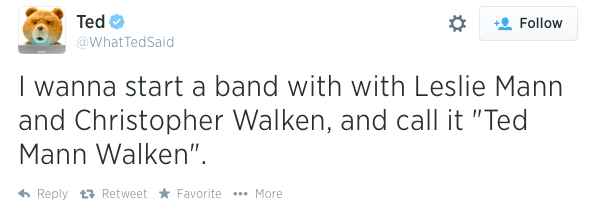
\includegraphics[width=10cm]{Ted}
  \caption[Unimportant Tweet]
   {Unimportant Tweet}
\end{figure}\leavevmode\\*
For a tweet such as the one above, we have no reason to provide Trustworthiness metrics or classification as the tweet serves no useful purpose and is purely someones opinion which does not affect anyone else personally or otherwise. \\*\\*
\noindent
We chose features from three different categories. We had $\textup{Message\_Based}$ Features, $\textup{User\_Based}$ Features and $\textup{Tweet\_Based}$ Features. In terms of $\textup{Message\_Based}$ Features, we initially only had \textit{tweet length, presence of URL, media type} and such generic details obtained from the Twitter API. The accuracy of predicting with purely the above features was slightly lower than the final accuracy we achieved. As can be seen our most successful model did perform well when it gave importance to features such as \textit{Emotions, Tweeting frequency} etc. However, now we have included and tested features like the emotion portrayed by the tweet (e.g, Happy, Sad, NoEmotion), the number of emoticons in the tweet and also, checks for keywords like `SHOCKING', `UNBELIEVABLE' etc. We observed that words of this nature were only used by accounts that were trying to gain the user attention, and truly Trustworthy profiles do not use such words to propagate information. We noticed slight improvements in prediction, with the incorporation of such detail. \\*\\*
Interestingly the accuracy of the prediction for the new data significantly increased when we filtered the training and testing datasets to either Happy or Sad tweets. This could be due to several reasons, one of which could be that if a tweet shows emotion in terms of smilies, then it has a higher tendency to be Untrustworthy than a tweet without smilies. This was one of the characteristics that we observed from the data that we gathered and has also been observed by Aditi Gupta et al. in \cite{11}. Hence training purely on tweets with emoticons we know that any of those tweets are Untrustworthy, hence predicting the rest as Trustworthy. This could also be due to the fact that a fair number of tweets with emoticons also consisted some of the reserved words such as `LEAKED', `REVEALED' etc. \\*\\*
We used several $\textup{User\_Based}$ features for our training however as mentioned earlier, the fact that we had only 45 listed users, and approximately 20,000 tweets from all of them. This meant constant repetition of user information throughout the training of data. We used the \textit{user location} as one of the parameters in our analysis however later realised that this does not produce accurate predictions. This may be due to the fact that we had a very small sample set of users from different countries.  So this would mean that if there was one profile from the Russia in our dataset and we had classified this profile as Untrustworthy then every other profile from Russia would also be graded slightly similarly depending on the weight given for location. We decided to drop this feature until we possessed a much larger user base to analyse. We thought that the \textit{length of the description string} for each user would be a good indication of how Trustworthy the profile is, however this was deemed unimportant by our Random Forest Classifier. We also noticed that the number of friends news profiles had was significantly lower than the number of people who followed these profiles. This was originally a concern as this could bias our analysis very much, however as we normalised the dataset this was not much of a problem. \\*\\* 
\noindent 
Below we suggest some future improvements to this model. We could further delve deeper and check the media associated to the message content, by verifying the validity of the URLs, Videos and Photos presented to us. For example, During the time when a Malaysian Airline MH370 initially went missing earlier this year, there were quite a few videos of the plane being found in some ocean or on land. One such example where a non working URL directing to a blank page, in the figure below:\\*\\*
\begin{figure}[hb]
  \centering
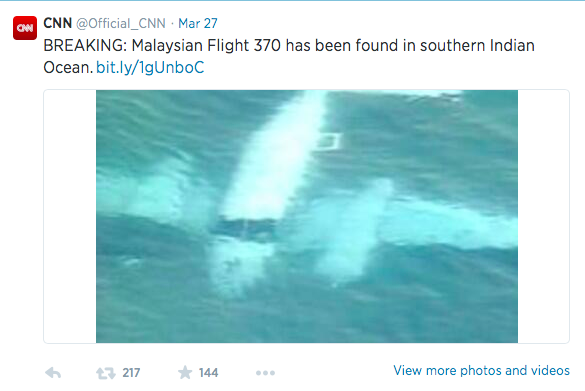
\includegraphics[width=10cm]{MalaysianAIrlines}
  \caption[MH370]
   {Malaysian Airlines Found in Southern Indian Ocean}
\end{figure}\leavevmode\\
\noindent
When clicking this URL, there appears to be no page linked to this. The user is also not the real CNN. In terms of videos posted, we could first check if a video exists at the location specified and secondly check the source of the video. We could also provide trust scores for some of the popular video streaming services such as YouTube, Vevo, YouView\footnote{\url{http://www.techradar.com/news/television/16-best-tv-streaming-services-1044010}} or news channels as opposed to an unknown website from which the video is available. Again this was apparent during the MH370 crisis where there were videos posted of planes in different oceans, most of which were either fake videos or non-existent links to videos.  Some other interesting features to measure in Message Content would be the amount of exclamation marks used, capitalisation and other special characters used. We could also go as far as analysing the profiles / trustworthiness scores of people that the current user has either mentioned or replied to in a message and factor that into our training. \\*\\*
\noindent
It would be interesting to perform some content based analysis for descriptions of user profiles as well as the names of the users, looking at key words and phrases. For example if we had checked the credibility of the name of the user for the tweet by \textit{falsenews} discussed above, we might have been able to avoid such classification mistakes. 
\section{Summary}
In this chapter we have highlighted the experiment conducted to assess the Trustworthiness metrics of Twitter. We have shown that the Random Forests Classifier worked best for most Tweets, but the Logistic Regression classifier provided a more generalised solution, in that its' ability to predict accurately tweets from general users. We have achieved 87\% and 97\% accuracies by Logistic Regression and Random Forests respectively. We have stated the most important features used in this analysis and provided examples to explain this further.  Our aim, was to learn features from known News Websites and known Untrustworthy websites and design a model that will predict a classifications which were accurate  at least 80\% of the time. From the discussion above, we have proved that our aim was met. In the next chapter we discuss some future improvements to the system and suggest a different approach to the problem as well as provide a conclusion.  